\chapter{系统评估}
\label{ch:evaluation}

本章给出本文两部分设计的定量结果。前半部分聚焦单节点 LKC-CXL-PIM，后半部分评估分布式 DisaggKV 系统。表~\ref{tab:results_summary} 总结了全文中使用的主要单节点结果。

\begin{table}[htbp]
\centering
\caption[单节点结果汇总]{基线与 LKC-CXL-PIM 的单节点定量结果汇总。}
\label{tab:results_summary}
\begin{tabular}{lcccc}
\toprule
\textbf{上下文长度} & \textbf{指标} & \textbf{基线} & \textbf{LKC-CXL-PIM} & \textbf{改进} \\
\midrule
\multirow{2}{*}{8K}   & Read Latency (M Cycles) & 10.77 & 0.12 & 89.7$\times$ \\
                      & Row Misses              & 80,483 & 1,195 & 67.3$\times$ \\
\midrule
\multirow{2}{*}{128K} & Read Latency (M Cycles) & 77.90 & 0.80 & 97.4$\times$ \\
                      & Row Misses              & 288,535 & 3,700 & 78.0$\times$ \\
\midrule
\textbf{Overall}      & Logic Area (Relative)   & 1.00 & 0.83 & 17\% Savings \\
\bottomrule
\end{tabular}
\end{table}

\section{单节点性能提升}

\begin{figure}[htbp]
\centering
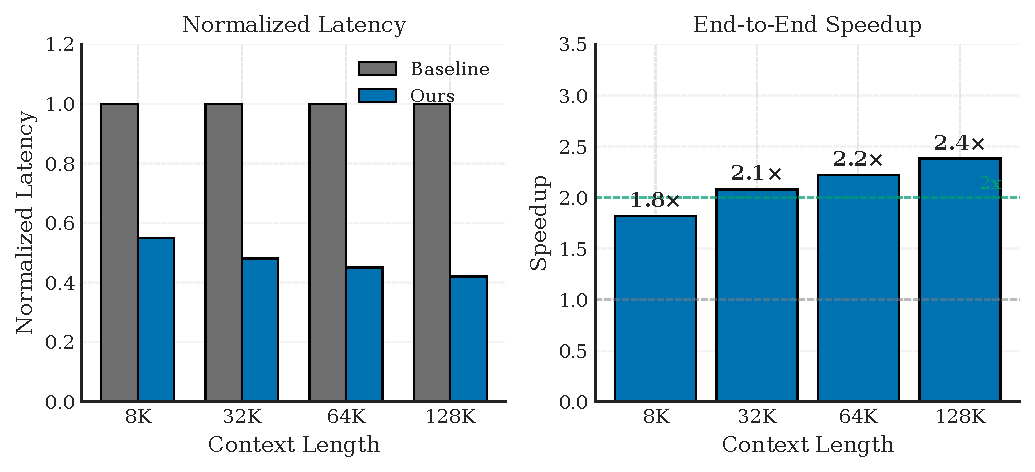
\includegraphics[width=\textwidth]{../paper_assets/figures/fig5_performance_speedup.pdf}
\caption[单节点 decode 加速比]{LKC-CXL-PIM 相对于主机聚合基线在不同上下文长度下的端到端 decode 加速比。}
\label{fig:performance_speedup}
\end{figure}

图~\ref{fig:performance_speedup} 给出了端到端 decode 加速比。随着上下文长度增加，近内存执行的优势更加明显，因为基线运行时间中用于搬移 KV 缓存的比例越来越高。测得加速比从 8K 时的 $1.8\times$ 上升到 128K 时的 $2.4\times$，说明该设计在基线愈发受带宽限制的场景中收益最大。

\begin{figure}[htbp]
\centering
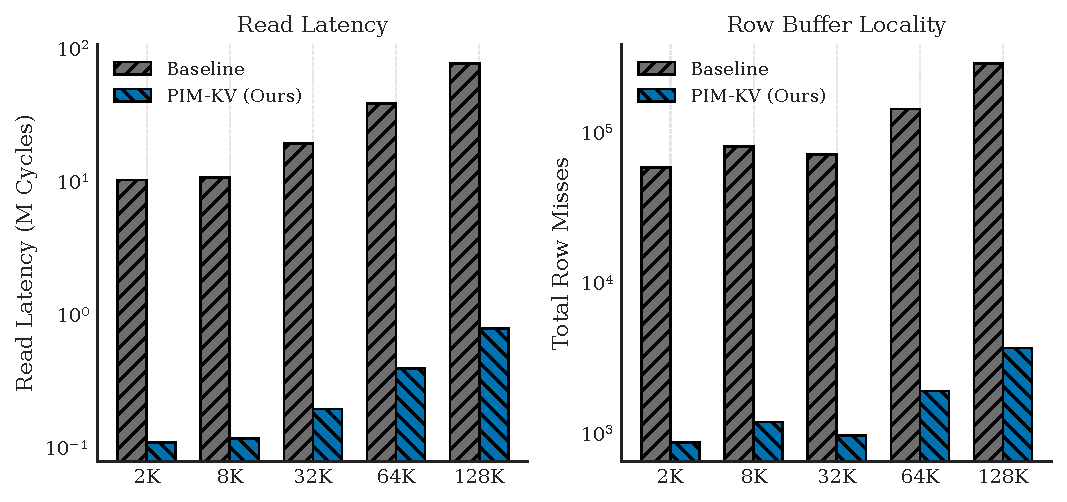
\includegraphics[width=0.9\textwidth]{../paper_assets/figures/fig7_ramulator_comparison.pdf}
\caption[周期级延迟对比]{基线与 LKC-CXL-PIM 在延迟组成和行缓冲局部性方面的周期级对比。}
\label{fig:ramulator}
\end{figure}

图~\ref{fig:ramulator} 进一步解释了这一加速来源。在 8K 上下文长度下，读取延迟从 10.77\,M cycles 降低到 0.12\,M cycles；在 128K 下，则从 77.90\,M cycles 降低到 0.80\,M cycles。相同的数据流重组还改善了行缓冲局部性：row misses 在 8K 时由 80,483 降为 1,195，在 128K 时由 288,535 降为 3,700。这与该设计的目标一致，即尽量将 KV 缓存访问留在内存设备内部，避免主机侧反复拉取。

\section{面积与能效}

\begin{figure}[htbp]
    \centering
    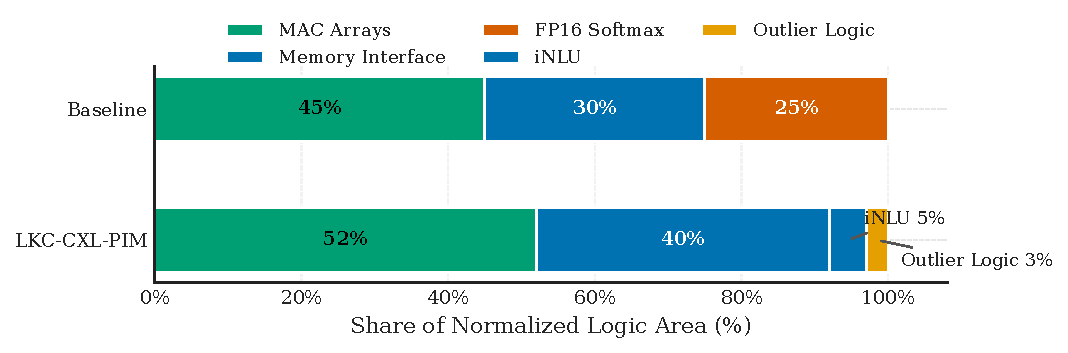
\includegraphics[width=0.92\textwidth]{../paper_assets/figures/fig6_area_breakdown.pdf}
    \caption[整体面积构成]{基线 Softmax 路径与 LKC-CXL-PIM 数据通路的整体逻辑面积构成。}
    \label{fig:area}
\end{figure}

图~\ref{fig:area} 给出了逻辑层级上的面积分解。在基线结构中，FP16 Softmax 模块约占逻辑预算的 25\%；而在 LKC-CXL-PIM 中，该模块被 iNLU 与异常值处理路径取代，两者合计约占 8\%，从而带来 17\% 的整体逻辑面积净缩减。

\begin{figure}[htbp]
    \centering
    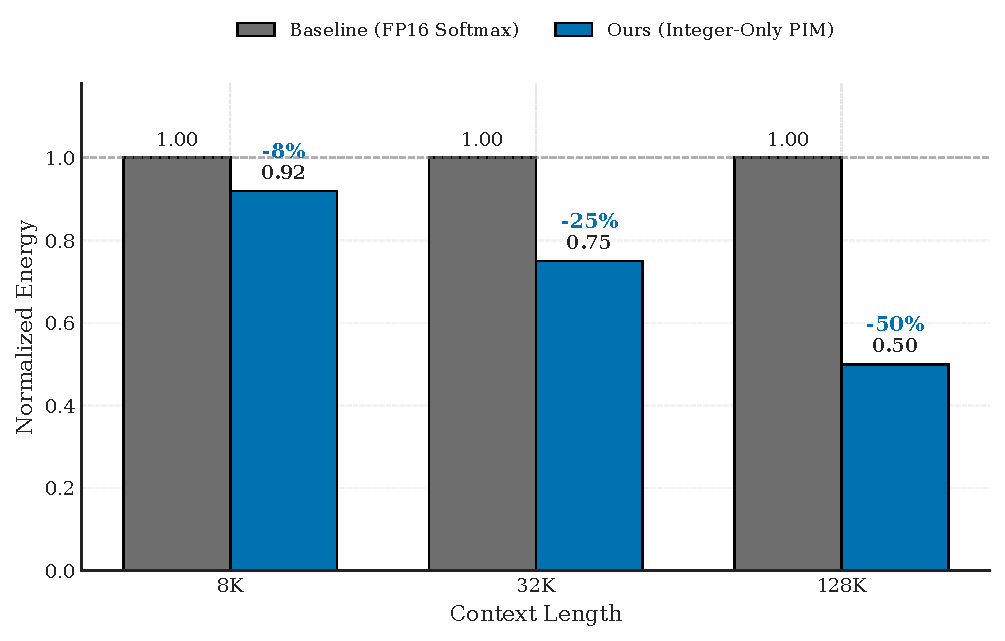
\includegraphics[width=0.78\textwidth]{../paper_assets/figures/fig2_energy_comparison.pdf}
    \caption[不同上下文长度下的归一化能耗]{代表性上下文长度下的归一化能耗对比。}
    \label{fig:energy}
\end{figure}

图~\ref{fig:energy} 展示了对应的能耗趋势。在 8K、32K 和 128K 上下文长度下，测得的归一化能耗节省分别为 8.3\%、24.9\% 和约 50.0\%。随着上下文长度增加，被避免的片外流量也不断增长，因此节省幅度相应扩大。

\section{iNLU 的数学保真度}

\begin{figure}[htbp]
    \centering
    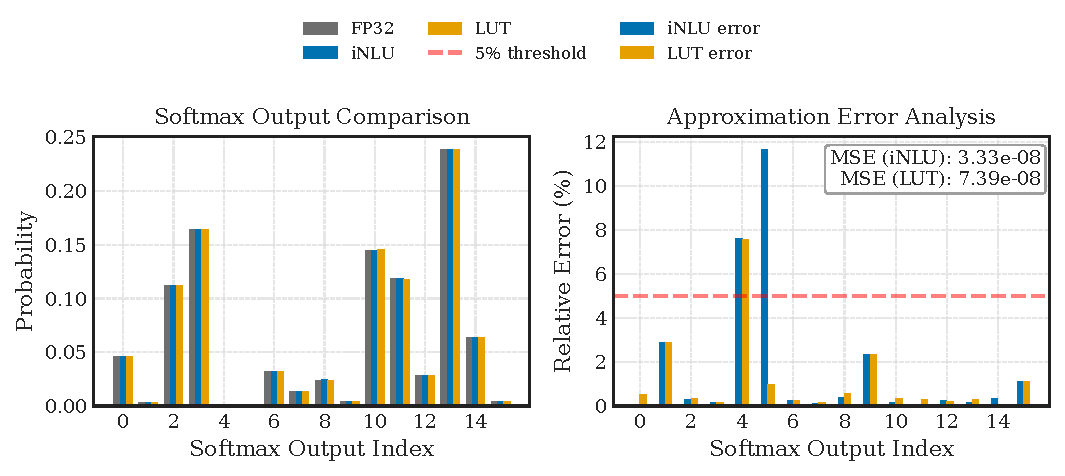
\includegraphics[width=0.9\textwidth]{../paper_assets/figures/fig4_inlu_accuracy.pdf}
    \caption[iNLU 的 Softmax 逼近精度]{iNLU 多项式路径与查找表近似在 Softmax 输出和逼近误差上的对比。}
    \label{fig:inlu_acc}
\end{figure}

\begin{figure}[htbp]
    \centering
    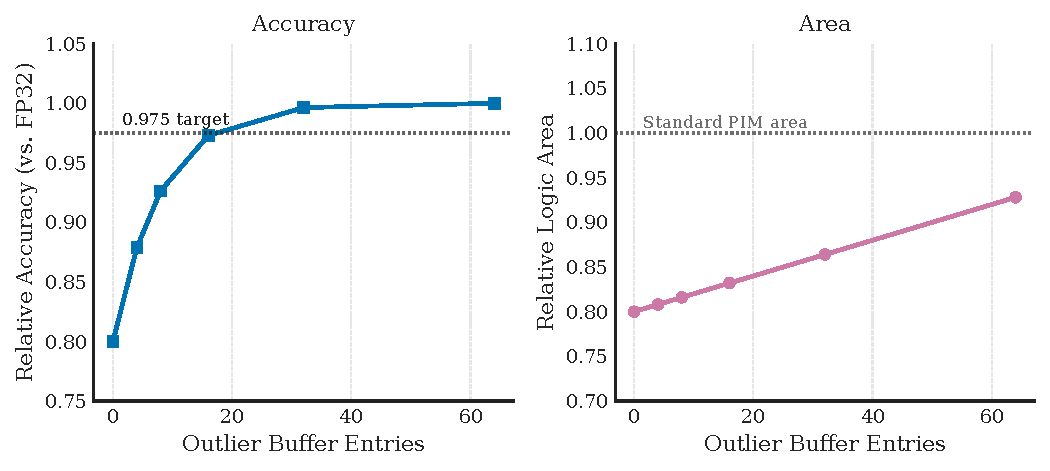
\includegraphics[width=0.9\textwidth]{../paper_assets/figures/fig10_sensitivity_outliers.pdf}
    \caption[异常值缓冲区灵敏度分析]{异常值缓冲区大小对相对精度与相对面积的影响。}
    \label{fig:sens_outliers}
\end{figure}

\begin{figure}[htbp]
    \centering
    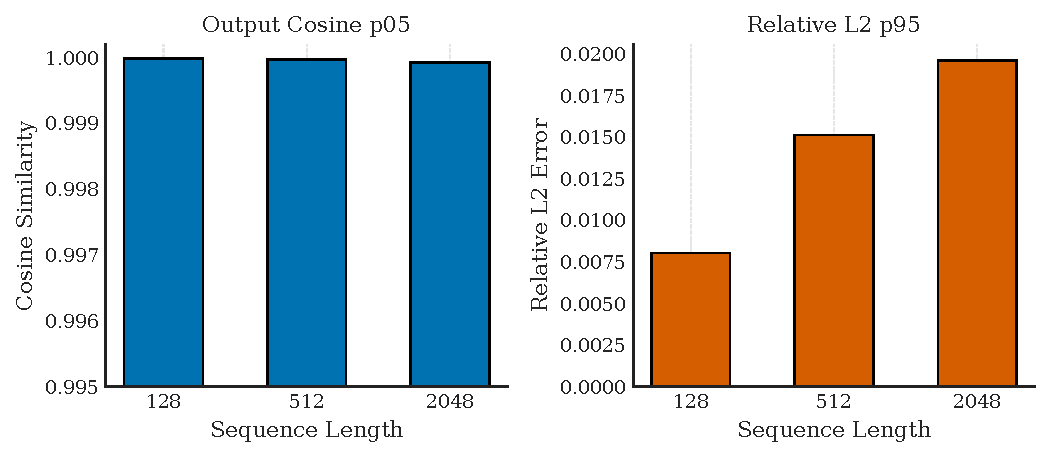
\includegraphics[width=0.78\textwidth]{../paper_assets/figures/fig11_attention_quality.pdf}
    \caption[定点 iNLU 下的注意力输出质量]{不同序列长度下定点 iNLU 路径的注意力输出质量。}
    \label{fig:attention_quality}
\end{figure}

图~\ref{fig:inlu_acc} 用于验证整数近似是否足以支持注意力归一化。图中的 iNLU 路径来自定点 golden model：logit 采用 Q10 表示，指数部分使用整数多项式路径，归一化输出采用 Q24 整数商。该路径能够较好地跟踪 FP32 参考结果，并且其均方误差低于图中给出的 64-entry 查找表替代方案（约为 $3.33\times10^{-8}$，而查找表为 $7.39\times10^{-8}$）。这说明 iNLU 的硬件缩减并非通过粗糙近似换取。

图~\ref{fig:attention_quality} 进一步将 Softmax 层面的误差与注意力行为联系起来。本文使用同一定点路径在一个轻量级单头 Q/K/V attention benchmark 中进行评估，序列长度覆盖 128、512 和 2048 tokens。每个序列长度下进行 128 次随机试验后，输出向量余弦相似度的最差 5 百分位仍高于 0.99992，而输出相对 $\ell_2$ 误差的最差 95 百分位为 1.96\%。这一实验不能替代完整语言模型 perplexity 评估，但说明整数归一化误差在 attention 输出层面仍保持较小。

图~\ref{fig:sens_outliers} 则评估了溢出路径的作用。纯 INT8 路径的相对精度起点约为 0.80，而 16-entry 缓冲区可将结果提升到约 0.97，同时相对面积大致仍与标准 PIM 基线相当。继续增加到 32 和 64 entries 可以进一步逼近完整精度，但 16 entries 之后的边际收益已明显小于相应面积开销，因此本文将 16-entry 缓冲区视为较为实际的工作点。

\section{多节点扩展性与吞吐}

\begin{figure}[htbp]
    \centering
    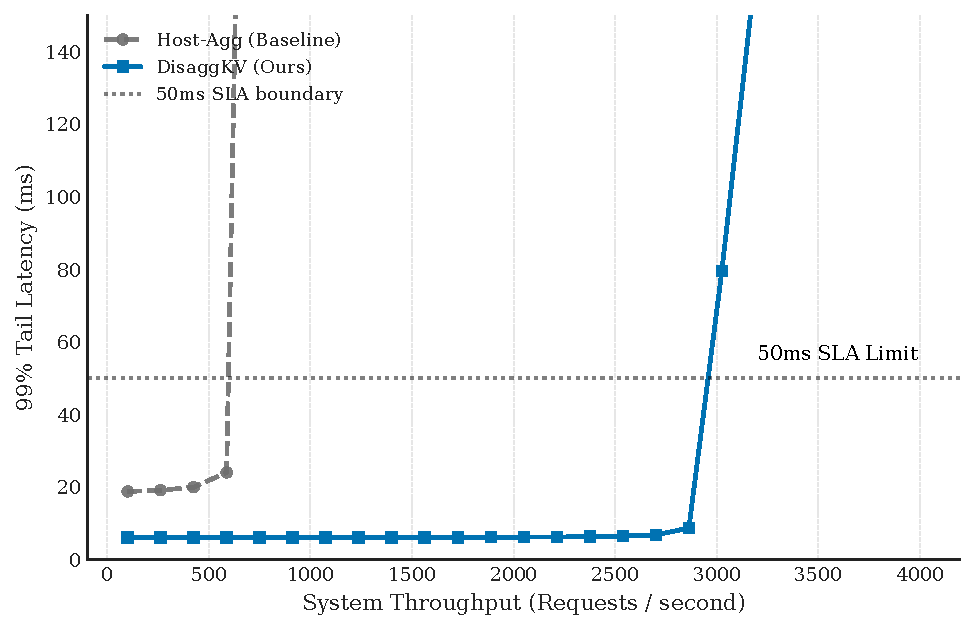
\includegraphics[width=0.82\textwidth]{../paper_assets/figures/fig1_throughput_latency.pdf}
    \caption[尾延迟与吞吐关系]{主机聚合基线与 DisaggKV 的尾延迟-吞吐关系。}
    \label{fig:throughput}
\end{figure}

图~\ref{fig:throughput} 基于第~\ref{ch:methodology} 章所述的校准排队模型，比较吞吐与 99 百分位尾延迟。主机聚合基线在略高于 600 requests/s 时越过 50\,ms 的 SLA 边界；而 DisaggKV 在 2.7K requests/s 之前始终保持低于 10\,ms，并直到略低于 3.0K requests/s 才越过 50\,ms 目标。以 SLA 边界为基准，这对应于相对于基线约 $4.5\times$ 的吞吐提升。

\begin{figure}[htbp]
    \centering
    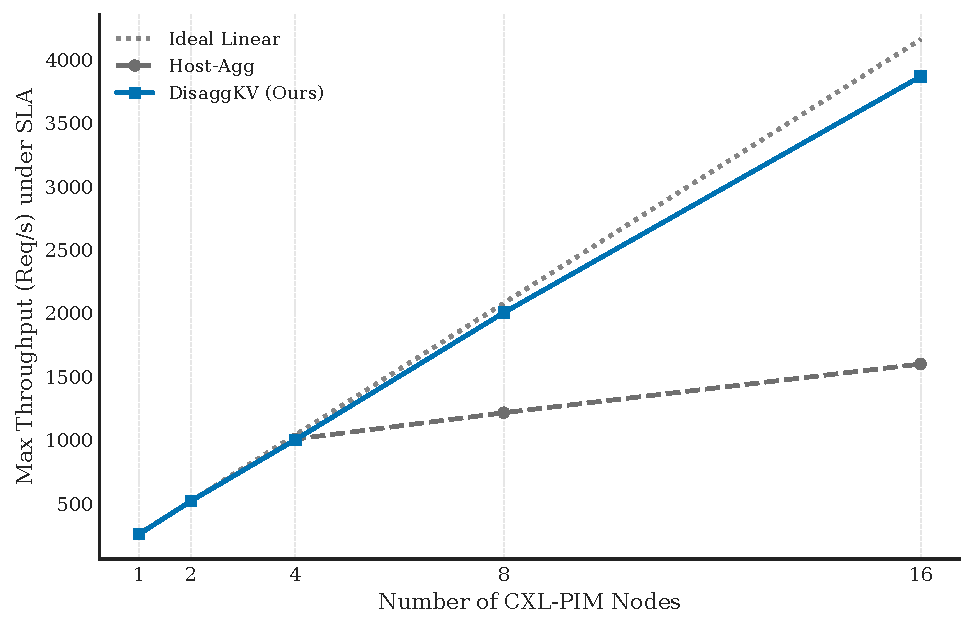
\includegraphics[width=0.82\textwidth]{../paper_assets/figures/fig2_scalability.pdf}
    \caption[分布式扩展性]{1 至 16 个节点下的分布式吞吐扩展。}
    \label{fig:scalability}
\end{figure}

图~\ref{fig:scalability} 展示了吞吐随 CXL 附加存储节点数的变化。吞吐从 1 个节点时的 257.4 requests/s 增长到 8 个节点时的 2004.9 requests/s，对应 $7.79\times$ 的提升。在 16 个节点时，吞吐达到 3867.7 requests/s，说明扩展仍在继续，但超过 8 个节点后边际收益开始更加明显地下降。

\section{网络流量降低与韧性}

\begin{figure}[htbp]
    \centering
    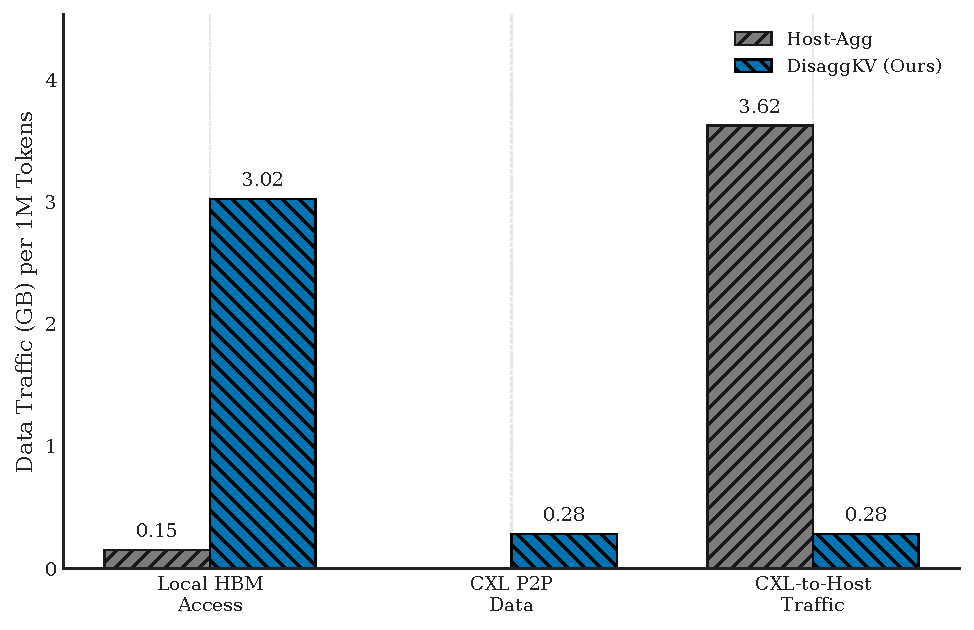
\includegraphics[width=0.82\textwidth]{../paper_assets/figures/fig3_network_breakdown.pdf}
    \caption[互联流量构成]{每 1M decoded tokens 对应的本地 HBM、点对点和面向主机流量分解。}
    \label{fig:network_break}
\end{figure}

图~\ref{fig:network_break} 给出了 DisaggKV 引入的流量权衡。由于更多工作在内存端点内部完成，本地 HBM 访问量有所增加。与此同时，面向主机的 CXL 流量从每 1M tokens 的 3.624\,GB 降低到 0.282\,GB，降幅达 92.2\%。若将点对点归约流量也一并计入，总互联流量仍相对于主机聚合基线下降约 84.4\%。这些数值由当前 CXL Fabric artifact 派生，并按照 50-request 踪迹的 token 数进行归一化。这正是 DisaggKV 能在达到 SLA 边界之前维持更高吞吐的核心原因。

\begin{figure}[htbp]
    \centering
    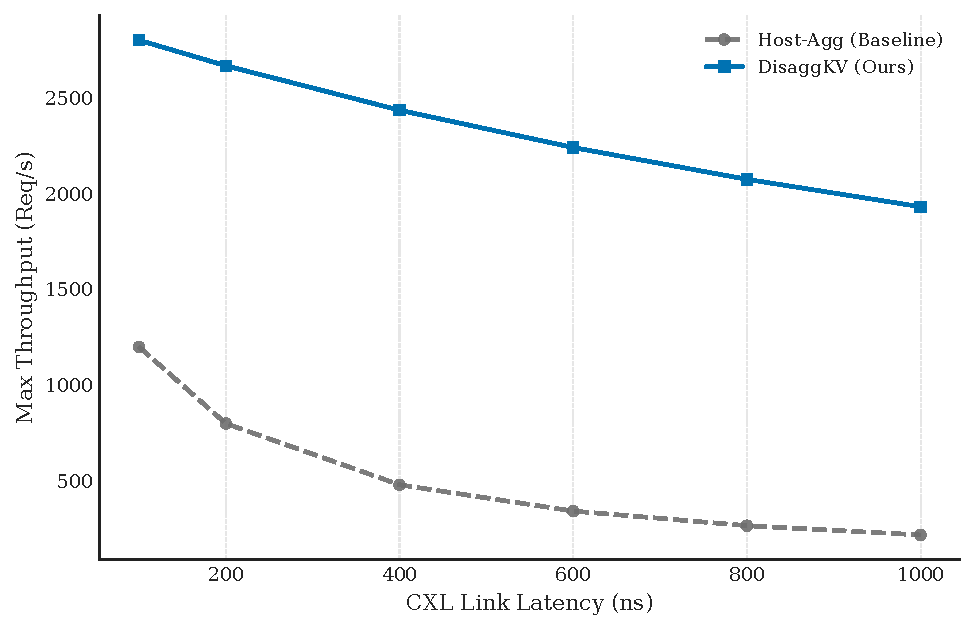
\includegraphics[width=0.82\textwidth]{../paper_assets/figures/fig5_sensitivity_latency.pdf}
    \caption[链路时延敏感性分析]{吞吐对 CXL 链路时延增加的敏感性。}
    \label{fig:sens_latency}
\end{figure}

图~\ref{fig:sens_latency} 评估了系统对 CXL 链路时延增加的敏感性。当链路时延从 100\,ns 增加到 1\,$\mu$s 时，主机聚合基线的吞吐从约 1200 requests/s 下降到约 230 requests/s；而 DisaggKV 则从约 2780 requests/s 下降到约 1930 requests/s。也就是说，DisaggKV 并非对时延完全不敏感，但由于其通信模式主要由紧凑标量归约而不是稠密张量拉取构成，因此对更长路径显著更具容忍性。

\begin{figure}[htbp]
\centering
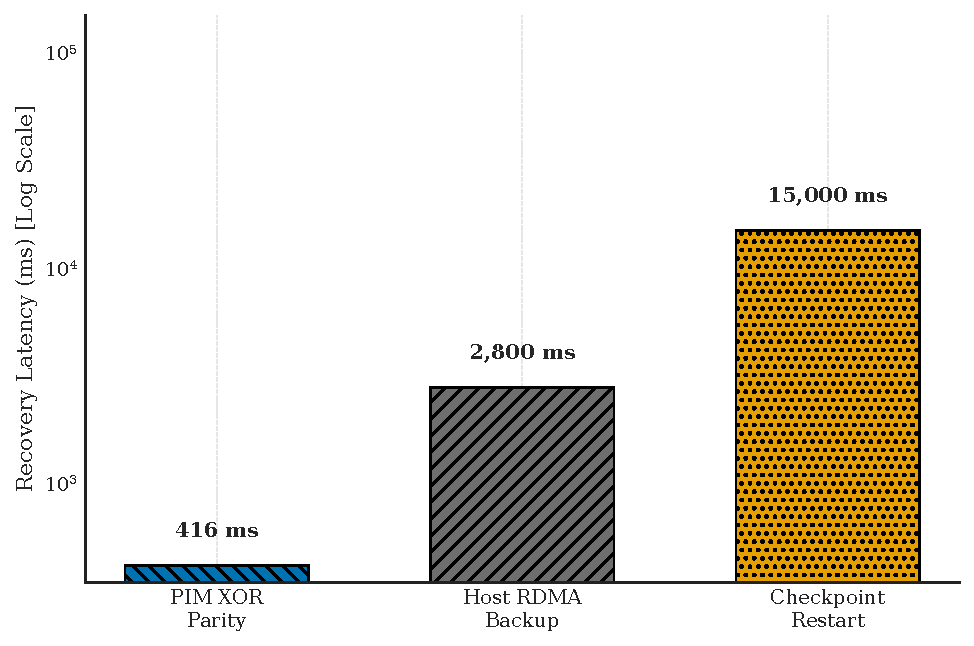
\includegraphics[width=0.78\textwidth]{../paper_assets/figures/fig4_fault_recovery.pdf}
\caption[故障恢复延迟对比]{本文奇偶辅助恢复方案与两种主机管理式恢复替代方案的故障恢复延迟对比。}
\label{fig:fault_recovery}
\end{figure}

图~\ref{fig:fault_recovery} 给出了故障注入模型下的韧性结果。基于奇偶辅助的 DisaggKV 恢复路径在故障注入 artifact 中达到 95 百分位 416.384\,ms；作为解析对比基线，主机级 RDMA 备份和 checkpoint-restart 恢复分别需要 2.8\,s 和 15\,s。由此可见，端点驱动的恢复机制不仅改善了故障隔离效果，也显著缩短了恢复时间，并避免了完整的主机侧重启。
